%%=============================================================================
%% Methodologie
%%=============================================================================

\chapter{\IfLanguageName{dutch}{Methodologie}{Methodology}}%
\label{ch:methodologie}

%% OK - In orde
%% BOK - Bijna in orde
%% NOK - Niet in orde

%% TODO: Hoe ben je te werk gegaan? Verdeel je onderzoek in grote fasen, en
%% licht in elke fase toe welke stappen je gevolgd hebt. Verantwoord waarom je
%% op deze manier te werk gegaan bent. Je moet kunnen aantonen dat je de best
%% mogelijke manier toegepast hebt om een antwoord te vinden op de
%% onderzoeksvraag.

% TODO - Inleiding - OK
In dit hoofdstuk wordt de Methodologie van het onderzoek beschreven en uitgelegd. Dit is deels een vervolgstuk op de technologieën die in de literatuurstudie besproken werden. Eerst en vooral komt een requirements-analyse en vooronderzoek aan bod, waaruit de potentiële kandidaten voor het onderzoek bekomen worden. In het vooronderzoek wordt een long list opgesteld waarvan. \\

Omdat Quivvy Solutions het belangrijk vindt up-to-date te blijven over diverse low-code platformen, hebben ze zelf reeds onderzoek gedaan naar een potentieel alternatief. Om die redenen is een van de kandidaten, Airtable, reeds gekozen uit de long list van kandidaten. Dit is één van de platformen waar het bedrijf veel interesse in heeft en graag zou laten onderzoeken. Desondanks het feit dat het reeds geselecteerd is, zal in het vooronderzoek de verschillende vereisten voor Airtable toch nog overlopen worden. \\


\subsection{Requirements-analyse}

De requirements voor een goed alternatief werden opgesteld aan de hand van de noden van Quivvy Solutions. Zij ontwikkelen low-code oplossingen voor kleine tot middelgrote bedrijven en gebruiken daarvoor voornamelijk Podio. De platformen moeten dus op zijn minst over de basisfunctionaliteiten van Podio beschikken. Bovendien moet er ook nagegaan worden of de alternatieven een goede toekomst hebben. Uiteindelijk werden de nodige vereisten verder opgedeeld in functionele en niet-functionele vereisten. \\

\textbf{Functionele vereisten:} % TODO FR - OK

\begin{itemize}
    \item De datastructuur moet bestaan uit een enkele database die zich als\textbf{`Single source of truth}` voordoet. Met andere woorden, het platform moet voor een applicatie een enkele database voorzien zodat alle data slechts op één plek wordt opgeslagen.
    \item Het platform moet over een bepaald minimum aan \textbf{flexibiliteit} bezitten. Dit betekent het zich niet mag focussen op specifieke use cases, maar dat het gebruikt kan worden voor elke context. Indien iets toch niet mogelijk is, moeten er workarounds of extensies aanwezig zijn die dit probleem verhelpen.
    \item Het platform moet in staat zijn om zaken zoals \textbf{workflows te automatiseren}.
    \item Het platform moet over een \textbf{eigen AP}I bezitten.
\end{itemize}

\textbf{Niet-functionele vereisten:} % TODO NFR - OK

\begin{itemize}
    \item Het platform moet \textbf{low-code/no-code} zijn.
    \item Het platform moet een stevige \textbf{gebruikersbasis} hebben. Dit betekent dat het minstens door ongeveer 250.000 gebruikers en 3000 bedrijven in gebruik moet zijn.
    \item Het platform moet \textbf{stabiel} zijn. Dit betekent dat het geen frequente storingen ondervindt en dat het zich beperkt tot maximaal twee incidenten per maand.
    \item Het platform moet \textbf{futureproof} zijn. Dit betekent dat het platform zeer sterk aan het groeien moet zijn. Hierbij wordt gekeken naar het aantal werknemers, de winst en de opgehaalde financiering op jaarbasis.
\end{itemize}


\subsection{Long list}
% - Tabel   nocode/ lowcode LONG LIST
\begin{table}[ht]
    \centering
    % TODO Add bron: https://analyticsindiamag.com/10-low-code-no-code-platforms-every-developer-should-know-of/ OK
    \caption{\label{tab:Tabel 3} Lijst met Podio alternatieven die onderzocht kunnen worden \autocite{Tasmia2022}.}
    \begin{tabular}{ | p{5cm} | p{2cm} | p{2cm} | }
        \hline
        \textbf{Platform}   & \textbf{Low-code} & \textbf{No-Code} \\
        \hline\hline
        Airtable            & ✓ & ✓ \\
        Appian              & ✓ & ✓ \\
        GoogleAppSheet      &    & ✓ \\
        Mendix              & ✓ & ✓ \\
        Notion              &    & ✓ \\
        Nintex              & ✓ & ✓ \\
        Shopify             & ✓ & ✓ \\
        Visual LANSA        & ✓ &    \\
        Kissflow            & ✓ &    \\
        Quixy               &    & ✓ \\
        ZohoCreator         & ✓ &    \\
        Caspio              &    & ✓ \\
        \hline
    \end{tabular}
    
    {\raggedright \textit{Opm. Er zijn nog alternatieven die niet in deze lijst vermeld staan.} \par}
\end{table}

\subsection{Short list}

Uit de long list werden Airtable en Google AppSheet gekozen, deze twee vormen samen de Short List voor het onderzoek. In de volgende 2 secties wordt de keuze voor deze kandidaten onderbouwd. 

\subsection{Airtable} % TODO - Airtable - BOK


% Low-code / Flexibel
Airtable is low-code en voorziet voorgemaakte templates voor tal van diverse use cases, zoals een `Product Catalog` of een `Customer Relationship Management (CRM)`. Daarnaast heeft de gebruiker natuurlijk ook de mogelijkheid om zelf een applicatie op te bouwen. Om die redenen kan het dus zeker als een flexibel platform beschouwd worden. \\
% TODO - https://www.softr.io/airtable/airtable-use-cases

% API / Automations
Zoals in de sectie \ref{subsec:airtable_web_API} werd vermeld, bevat Airtable ook een krachtige API die het verkrijgen, aanmaken, updaten en verwijderen van een of meerdere records voorziet. Vervolgens zijn ook automatisaties mogelijk met Airtable. Via triggers kan men verschillende soorten actions automatisch laten uitvoeren. \\
% TODO - https://airtable.com/developers/web/api/introduction (al aanwezig in bibtex)
% TODO - https://support.airtable.com/docs/getting-started-with-airtable-automations

% Futureproof
Toen het bedrijf in 2013 begon, had het minder dan 10 werknemers en was er slechts 3 miljoen dollar aan financiering beschikbaar. Maar tegen het einde van 2021 had Airtable aanzienlijke vooruitgang geboekt: het beschikte op dat moment ongeveer over 700 werknemers en wist maar liefst één miljard dollar aan financiering op te halen. Dit is een enorme verbetering ten opzichte van het voorgaande jaar, waarin slechts 185 miljoen dollar werd opgehaald. Bovendien werd in 2021 de waarde van Airtable geschat op 11,7 miljard dollar, wat ongeveer 5 miljard meer is dan in 2020. Ten slotte is de jaarlijkse groei van het bedrijf is ongeveer 39\% en brengt het maandelijks meerdere updates uit. Uit voorgaande informatie kan dus besloten worden dat het platform zeker futureproof is. \\
% TODO - https://www.mksguide.com/airtable-user-and-company-stats/
% TODO - Invoegen Airtable_Valuation_2018_To_2021.png

% Stabiel
Airtable heeft de afgelopen 2 jaar (januari 2021 tot december 2022) gemiddeld 1 à 2 incidenten per maand gehad, deze incidenten werden meestal ook de dag zelf nog opgelost . Het voldoet dus aan de vastgelegde requirement. \\
% TODO - https://status.airtable.com/history

% Gebruikersbasis
Airtable wordt gebruikt door meer dan 300.000 bedrijven, waaronder Shopify, Nike en AT\&T. Bovendien gebruikt 80\% van de `Fortune 100`\footnote{Groep met de 100 grootste bedrijven van de Verenigde Staten} het platform. Vervolgens heeft meer dan 30\% van de klanten zich ingeschreven voor een betaald plan. \\
% TODO - https://nira.com/companies-that-use-airtable/


\subsection{AppSheet} % TODO - keuze AppSheet - NOK

% Low-code / Flexibel
De tweede kandidaat voor het onderzoek is het no-code platform Google AppSheet. Het voorziet een groot aantal voorgemaakte templates of 'sample apps' die voor verschillende use cases gebruikt kunnen worden. Alhoewel het platform in het algemeen minder flexibel is dan Podio of Airtable, voldoet het wel aan de requirement. Verder heeft het platform ook een eigen API, maar deze is iets minder uitgebreid dan diegene van Airtable of Podio \\

Daarnaast wordt het platform vaak gebruikt door organisaties met meer dan 10.000 werknemers. Meta Platforms, Inc.\footnote{https://www.meta.com/} of kortweg Meta, het Amerikaans moederbedrijf van ondere andere facebook, is maakt bijvoorbeeld gebruik van AppSheet. Verder is het platform geïntegreerd met Google Workspace en wordt ervan verwacht dat het blijft groeien. Bovendien heeft Google Workspace in 2022 aangekondigd dat ze van plan zijn om te investeren in cursussen en opleidingen voor AppSheet. Uit voorgaande informatie kan dus besloten worden dat AppSheet ook een futureproof platform is. \\ 

Vervolgens kan er besloten worden dat AppSheet voldoet aan de stabiliteits-requirement. Sinds begin 2023 heeft het platform nog maar één keer down time gehad, namelijk in januari 2023. \\
%TODO - https://www.saashub.com/appsheet-status

Ten slotte zijn ook tal van automatisaties mogelijk via AppSheet, die in het platform 'bots' genoemd worden. \\
%TODO - https://workspace.google.com/blog/product-announcements/hidden-secret-open-secret-year-ahead-appsheet



\section{De uit te bouwen Use Case} % TODO - OK

Als use case werd in samenspraak met Quivvy Solutions gekozen voor een eenvoudige applicatie die een simpel stageproces bijhoudt. Ten eerste moet er dus een lijst met studenten en hun gegevens bijhouden worden. Bovendien moet elke student gelinkt zijn aan een dossier, waar verschillende zaken aan vast hangen zoals onder andere een toegewezen begeleider, sollicitaties die de student gedaan heeft, evaluaties gegeven door een begeleider, een toegewezen stageopdracht en een totaal score voor het dossier. Hieruit volgt dus dat er ook andere lijsten zoals docenten, sollicitaties,$\ldots$ aanwezig moeten zijn binnen de applicatie. Daarnaast heeft een student ook een richting die dan op zich meerdere specialisaties bevat, dit zijn ook elementen die als lijst moeten worden opgeslagen. Vervolgens moet er ook de mogelijkheid zijn om het dossier eenvoudig om te vormen naar een PDF bestand. Hiermee is het concept van de use case toegelicht, een verdere uitwerking volgt in de analyse fase van het onderzoek. \\

\newpage

\section{Onderzoek} 
In deze sectie wordt het effectieve onderzoek besproken, waarbij wordt beschreven hoe de use case is ontwikkeld op verschillende platformen en in hoeverre dit voldeed aan een reeks criteria. De criteria voor het onderzoek zijn als volgt geformuleerd;

\begin{itemize}
    \item Hoe eenvoudig is het om \textbf{relaties} te leggen tussen verschillende onderdelen, bijvoorbeeld tussen een studierichting en zijn specialisaties?
    \item Is het mogelijk om een studentendossier \textbf{automatisch om te vormen} naar een PDF met de nodige informatie? Indien wel, hoe gemakkelijk lukt dit?
    \item Is het mogelijk om via \textbf{workflows} sollicitaties/stageopdrachten aan te maken en deze automatisch te linken met de overeenkomstige student/bedrijf?
    \item Hoe eenvoudig is het om \textbf{calculaties} of berekeningen uit te voeren, zoals een overzicht opstellen van de verschillende stageopdrachten die een bedrijf voorziet?
    \item Hoe aangenaam is de \textbf{gebruikerservaring}? Met name hoeveel keer moet men klikken of navigeren om een bepaald doel te bereiken? Is de tool eenvoudig te gebruiken of is de bediening eerder complex?
    \item Hoe intuïtief is de \textbf{user interface (UI)}? Is deze overzichtelijk of staan er veel zaken door elkaar? Hoe eenvoudig kan een bepaalde functie terug gevonden? Kunnen activiteiten gemakkelijk opgevolgd worden, bijvoorbeeld via dynamische views of tegels?
    \item Hoe \textbf{probleemloos} verloopt het uitbouwen van de use case? Welke problemen komt men allemaal tegen?
\end{itemize}

\subsection{Analyse Use Case}

Net zoals bij andere IT projecten is het belangrijk om eerst een analyse uit te voeren voordat er effectief gestart wordt met ontwikkelen. De analyse voor een use case kan verschillen afhangend van het platform waarvoor men ze wil uitvoeren. Aangezien deze studie alternatieven zoekt voor Podio, wordt de analyse fase uitgevoerd in functie van Podio en daarna toegepast op Airtable en Google AppSheet. \\

In Podio wordt een database tabel voorgesteld als een app, die informatie over een bepaald onderwerp bijhoudt. Uit de beschrijving van de use case kan afgeleid worden er op zijn minst 9 apps aanwezig moeten zijn, namelijk studenten, bedrijven, docenten, stageopdrachten, sollicitaties, richtingen, specialisaties, studentendossiers en evaluaties. \\

Het is belangrijk om in te zien dat studenten en docenten beide personen zijn en dat een bedrijf ook meerdere contactpersonen kan hebben. Om een persistente structuur te hebben, is er dus een 10de app genaamd ‘Contacten’ nodig. Bovendien voorkomt dit ook eventuele redundante data. Een docent kan bijvoorbeeld contactpersoon zijn bij een bedrijf, maar dit kan moeilijk aangetoond worden, aangezien er geen expliciete relatie is tussen ‘Bedrijven’ en ‘Docenten’. Deze persoon zou dus twee keer moeten opgeslagen worden in de databank, wat tegenin de richtlijnen van Podio gaat. \\

Daarnaast moet er ook rekening gehouden worden met het leggen van relaties tussen de verschillende apps. In Podio is het bij het 1-op-1 relaties en 1-op-veel relaties beter om de relatie bij slechts één van de twee te apps leggen en bij de andere een calculatie veld te gebruiken. Anders kan er verwarring ontstaan binnenin het platform, indien er bijvoorbeeld een item verwijderd wordt kan de relatie aan één van de kanten nog steeds bestaan. \\

Tenslotte is het belangrijk om na te denken welke automatisaties allemaal toegepast kunnen worden. In dit onderzoek wordt er beperkt tot de volgende;

\begin{itemize}
    \item Automatisch aanmaken van een sollicitatie en linken aan een dossier.
    \item Automatisch aanmaken van een evaluatie en linken een dossier.
    \item Automatisch aanmaken van een stageopdracht en linken aan een bedrijf.
    \item Automatisch invullen van richting wanneer een specialisatie wordt gelinkt aan een stageopdracht.
    \item Automatisch aanmaken van een specialisatie en linken aan een richting.
    \item Dossier automatisch omvormen tot een opgemaakt pdf-bestand.
\end{itemize}

\begin{table}
    \centering
    \caption{\label{tab:Resultaat analyse} }
    \begin{tabular}{ | p{4cm} | p{8cm} | }
        \hline
        \textbf{App} & \textbf{Attributen} \\
        \hline\hline
        Contacten       & (calc.\footnote{calculatie}) ID, voornaam, familienaam, adres, geboortedatum, email, telefoonnummer, (calc.) Bedrijven \\
        Studenten       & (calc.) ID, (rel.\footnote{relatie}) Contact, (rel.) Studierichting, (rel.)  Specialisatie, klasgroep \\
        Bedrijven       & (calc.) ID, naam, adres, email, telefoonnummer, link, (rel.) Contactpersonen, (calc.) Stageopdrachten \\
        Docenten        & (calc.) ID, rol, (rel.) Studierichting \\
        Stageopdrachten & (calc.) ID, titel, (rel.) Bedrijf, beschrijving, (rel.) Richting, (rel.) Specialisaties, periode, aantal-studenten, (rel.) Toegewezen-aan \\
        Sollicitaties   & (calc.) ID, (rel.) Student, (rel.) Bedrijf, datum-gesprek, alleen/medestudent, (rel.) Medestudent, resultaat, opmerking \\
        Richtingen      & (calc.) ID, naam, afkorting, status, (calc.) Specialisaties \\
        Specialisaties  & (calc.) ID, naam-specialisatie, (rel.) Richting \\
        Dossiers        & (calc.) ID, Titel, (rel.) Student, (rel.) Begeleider, (rel.) Sollicitaties, (rel.) Evaluaties, (rel.) Toegewezen-stageopdracht, (calc.) Score \\
        Evaluaties      & (calc.) ID, datum, (rel.) Student. \\
        \hline
    \end{tabular}
\end{table}

Nu de analyse fase voltooid is kan er gestart worden met het ontwikkelen in Podio, Airtable en Google AppSheet. Vervolgens wordt voor elk van de platformen nogmaals de criteria overlopen en wordt er toegelicht hoe goed elk platform eraan voldoet. \\

\newpage



% PODIO __________________________________________________________________________________________________________________________
\subsection{Podio} % TODO - Podio - OK

Vooraleer het bouwproces wordt toegelicht is het belangrijk om nog eens de structuur van Podio op te frissen. In Podio wordt een use case of project weergegeven aan de hand van een workspace. Deze workspace bevat één of meerdere apps die een template voorzien voor een bepaald onderdeel. Een template wordt gebruikt om een item van de app op te bouwen en is een samenstelling van velden zoals een tekstveld, datumveld of calculatieveld. Vanuit een database-perspectief kan een workspace dus gezien worden als de database, een app als een tabel, een template als de kolommen van de tabel en een item als een rij in een tabel. \\

In Podio is de eerste stap van het ontwikkelingsproces dus het aanmaken van de workspace waarin alles gebouwd zal worden. De ‘Activity’ app, zie figuur \ref{fig:meth_podio_workspace}, wordt standaard aangemaakt bij het creëren van een workspace en bevat een overzicht van wat er zich allemaal afspeelt. Indien iets wordt aangepast, wordt dit weergegeven in een tijdslijn samen met de persoon die het heeft aangepast en wanneer de aanpassing verricht werd. Daarnaast wordt ook een kalendertegel en een lijsttegel, met taken die zelf toegevoegd kunnen worden, voorzien. Bovendien is er de optie om zelf tegels toe te voegen die data uit de workspace kunnen weergeven. \\

\begin{figure}[ht]
    \centering
    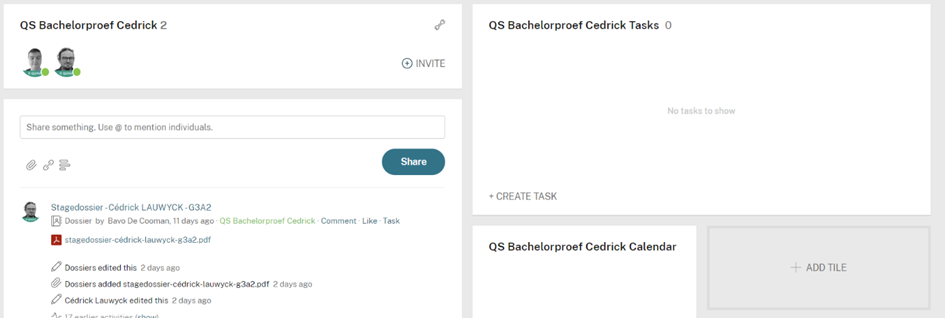
\includegraphics[width=\linewidth]{methodologie/Podio_workspace.png}
    \caption{'Activity' app in een Podio workspace.}
    \label{fig:meth_podio_workspace}
\end{figure}

Nadat de workspace is aangemaakt, kan voor elk onderwerp uit de analyse een app aangemaakt worden. Het is voordeliger om eerste alle apps aan te maken vooraleer de attributen worden toegevoegd, want men kan namelijk geen relatie leggen naar iets dat nog niet bestaat. Dit kan eenvoudig gedaan worden door op de ‘Add App’-knop te klikken, waarna een venster getoond wordt die vraagt achter de naam van de app, de naam van een item en icoon. Voor de benamingen wordt door Quivvy vaak enkelvoud en meervoud gebruikt, ter illustratie: de ‘Contacten’ app heeft ‘Contact’ als naam van het item. Het icoon daarentegen kan gekozen worden uit een uitgebreide lijst van iconen. Het uiteindelijke resultaat van deze stap wordt weergegeven in figuur \ref{fig:meth_podio_lijstApps}. \\

\begin{figure}[ht]
    \centering
    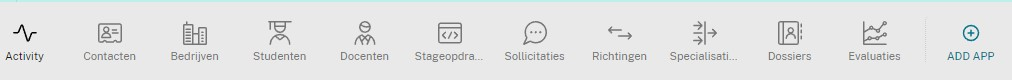
\includegraphics[width=\linewidth]{methodologie/Podio_lijstApps.jpg}
    \caption{Aangemaakte apps in de Podio workspace.}
    \label{fig:meth_podio_lijstApps}
\end{figure}

Eens alle apps aangemaakt zijn, is de fundering van de use case afgewerkt. Nu kan er over gegaan worden tot het instellen van de verschillende attributen en relaties. Dit is mogelijk in 2 simpele klikken, namelijk door naar de app te navigeren en vervolgens via het ‘moersleutel’-icoontje de verschillende instellingen van de openen. Daarna kan men via een derde klik de template van de app gaan bewerken. Zoals eerder vermeld is een template een samenstelling van verschillende types velden die Podio voorziet. Voor de use case wordt dus elk voor elk attribuut van de app een veld toegevoegd. Ter illustratie wordt in figuur \ref{fig:meth_podio_dossierTemplate} de uitgewerkte template voor de 'Dossiers' app van de use case weergegeven. Eerst een vooral werd een calculatieveld toegevoegd voor de ID van het dossier. In dit veld komt het low-code gedeelte van Podio aan bod, het veld accepteert namelijk JavaScript en kan op allerlei manieren gebruikt worden. De laatste lijn in het calculatie veld is wat er uiteindelijk wordt weergegeven, daaronder is ook een preview zichtbaar. In het geval van een dossier wordt een stuk tekst samengevoegd met de ID van de student. Vervolgens wordt een simpel tekstveld gebruikt voor de titel van het dossier, gevolgd door 2 relatievelden om de student en begeleider te linken. Daarna wordt een categorieveld ingevoegd met de opties `Evaluatie` en `Sollicitatie`, dit zal later gebruikt worden voor het toevoegen van een evaluatie of sollicitatie via automatisaties. Podio voorziet namelijk geen knop velden, om die reden wordt een categorie veld gebruikt als workaround. Verder worden nog 2 relatievelden toegevoegd en nog een calculatieveld waarin de totaalscore van de evaluaties wordt uitgerekend en weergegeven. Het is belangrijk om te vermelden dat er voor elk een set van opties beschikbaar zijn, om bijvoorbeeld het veld verplicht te maken of om het aantal relaties in een relatieveld te beperken. \\

\begin{figure}[ht]
    \centering
    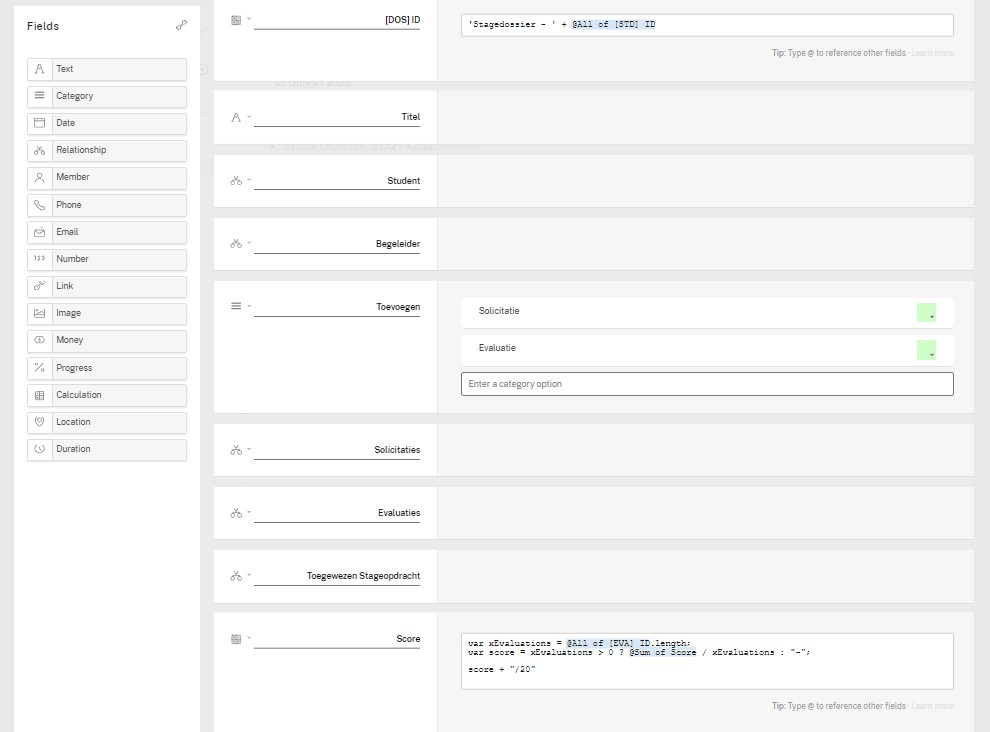
\includegraphics[width=\linewidth]{methodologie/Podio_dossierTemplate.jpg}
    \caption{Uitgewerkte template van de 'Dossier' app.}
    \label{fig:meth_podio_dossierTemplate}
\end{figure}

Om de data mooi weer te geven wordt als extra ook de layout aangepast. Podio voorziet standaard 5 verschillende layouts, namelijk 'Badge', 'Table', 'Card', 'Activity' en 'Calender', verder kunnen ook nog filters ingesteld worden op de attributen van een app. Eens alles geconfigureerd is naar keuze kan ten slotte de weergave als view worden opgeslagen. In figuur \ref{fig:meth_podio_badgeLayout} is een voorbeeld van de badge layout te zien. Bovendien kan men voor elke app via de 'Layout options' selecteren welke velden men wil weergeven op een individuele badge. \\

\begin{figure}[ht]
    \centering
    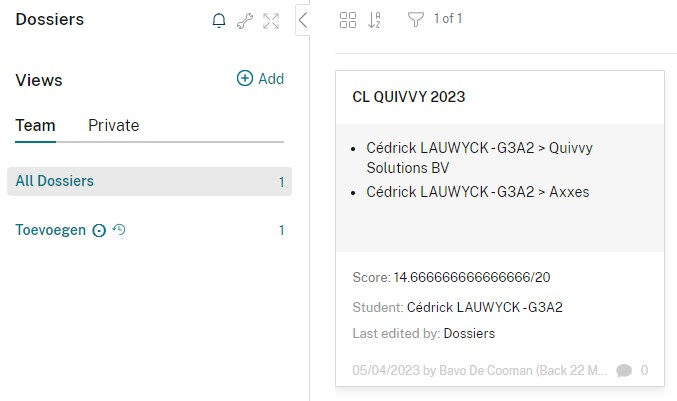
\includegraphics[width=\linewidth]{methodologie/Podio_badgeLayout.jpg}
    \caption{Badge layout in Podio.}
    \label{fig:meth_podio_badgeLayout}
\end{figure}

De volgende stap is om de automatisaties of workflows toe te voegen, dit gebeurt via Globiflow\footnote{wordt ook wel Citrix Podio Workflow Automation genoemd.}, een geavanceerde workflow automation tool gemaakt voor Podio. Door naar de instellingen van een willekeurige app te navigeren en vervolgens door te klikken op `workflow automations`, wordt men omgeleid naar een externe pagina waar automatisaties kunnen worden ingesteld. Eerst en vooral is het belangrijk om onderaan de pagina op de 'Refresh from Podio' knop te klikken, deze zorgt er namelijk voor dat de laatst opgeslagen configuratie van de Podio workspace wordt opgehaald. Nu alle apps en bijkomende velden aanwezig zijn, kunnen er workflows aangemaakt worden. Deze bevatten een trigger, een set van filters en een set van acties die worden uitgevoerd. Er zal dus voor elke automatisatie in de analyse, een workflow aangemaakt worden. Een handige feature van Globiflow, is dat het voor elke workflow ook een verkorte versie of recept weergeeft. Bovendien wordt ook een schatting weergegeven van hoeveel minuten er bespaard worden door de workflow uit te voeren. \\

In figuur \ref{fig:meth_podio_workflow} is terug een uitgewerkt voorbeeld te zien, namelijk het omvormen van een dossier tot pdf bestand. De trigger voor deze workflow is het updaten van een dossier, in de filters wordt dit dan verfijnd tot het updaten van het 'verwerken' veld. Eens dit op `Omzetten naar PDF` wordt gezet, zal de flow verdergaan naar de acties, bij een andere waarde wordt de flow beëindigt. Bij de eerste actie wordt een variabele opgeslagen met het jaartal van creatiedatum van het dossier, deze zal dan later gebruikt worden in de template voor het omvormen naar PDF. Vervolgens wordt de data van enkele referenties opgehaald, namelijk de informatie over de student, studierichting en het bedrijf. Daarna komt het omzetten naar PDF bestand, men kan volledig zelf een template opbouwen met alle nodige informatie uit Podio. Bovendien is het ook mogelijk om een footer en header in te stellen, voor onze use case wordt in de footer bijvoorbeeld informatie over Hogeschool Gent weergegeven. Er hoeft geen actie toegevoegd te worden om de gemaakte PDF aan het item zelf te hangen, want dit zit namelijk inbegrepen in de actie. Indien men het bestand zou willen doormailen kan dat eenvoudig door vanuit deze workflow een andere workflow te activeren en vervolgens de PDF mee te geven. De voorlaatste stap van automatisatie is het `Dossier` item terug updaten om het 'Toevoegen' veld terug op leeg te zetten. Ten slotte worden nog enkele acties toegevoegd om de referenties die eerder werden opgehaald terug op te ruimen, eens dit gebeurt is, is de workflow afgewerkt. \\

\begin{figure}[ht]
    \centering
    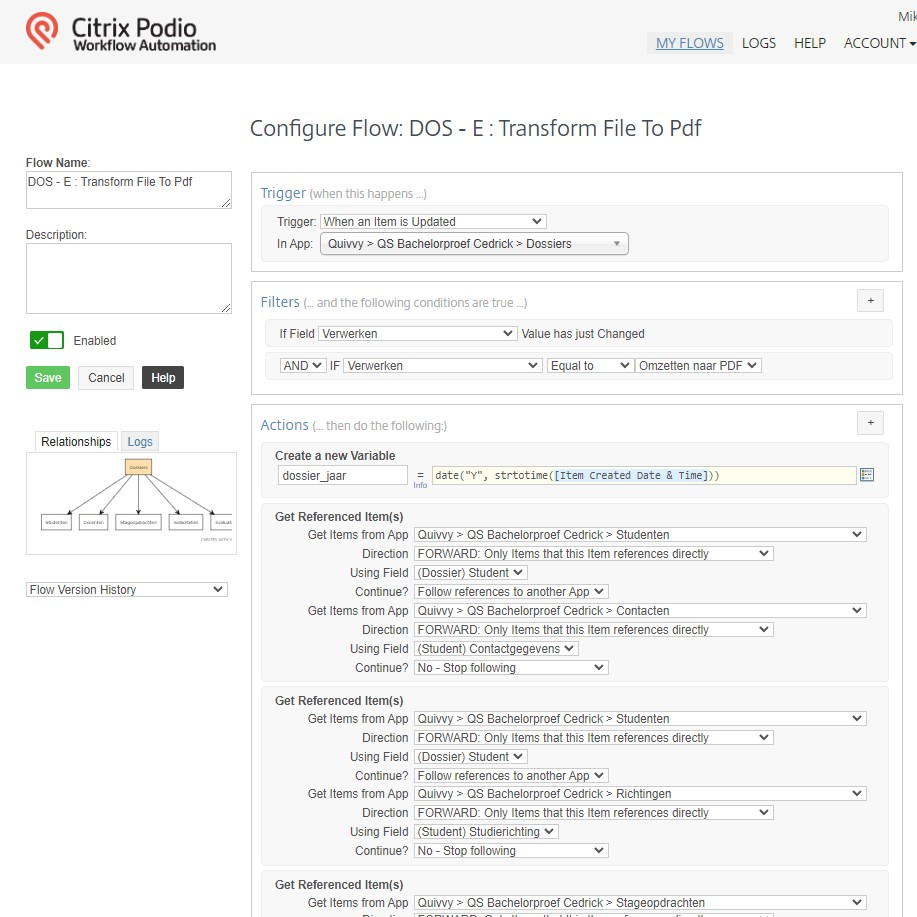
\includegraphics[width=\linewidth]{methodologie/Podio_workflow.jpg}
    \caption{Workflow in Globiflow.}
    \label{fig:meth_podio_workflow}
\end{figure}

Nu de use case is voltooid in Podio, is het belangrijk om de criteria eens door te nemen en kort te evalueren hoe goed het platform presteert. Allereerst is het heel eenvoudig om relaties te leggen via het relatieveld, hoewel er wel altijd nagedacht moet worden aan welke kant de relatie wordt gelegd. Ten tweede kunnen workflows ook gemakkelijk worden ingesteld. Alles heeft een duidelijke benaming, waardoor zelfs lange reeksen van acties eenvoudig te begrijpen zijn. Bovendien biedt Podio een zeer prettige gebruikerservaring. De verschillende knoppen en functies zijn gemakkelijk te begrijpen en kunnen met slechts 1 tot 4 klikken worden bereikt. \\

Het uitbouwen van de use case is echter niet zonder problemen verlopen. Bijvoorbeeld, het instellen van de 'layout options' voor een badge moest vaak twee keer worden toegepast, omdat ze de eerste keer niet werden opgeslagen in het systeem. \\

\newpage



% AIRTABLE __________________________________________________________________________________________________________________________
\subsection{Airtable} % TODO - Airtable - OK

Nu de use case uitgewerkt is in Podio kan overgegaan worden naar het eerste potentiële alternatief, Airtable. De structuur van Airtable is gelijkaardig aan die van Podio, ook hier wordt weer gewerkt met workspaces. In een workspace kan dan een base of database worden aangemaakt, deze zal alle data van de use case omvatten. Verder bestaat een base uit zogenaamde `Tables` of tabellen, die vergelijkbaar zijn met apps uit Podio of dus met een tabel in een database. Voor elk onderwerp uit de analyse wordt dus een tabel toegevoegd, de attributen of kolommen zullen later ingesteld worden. Bij het aanmaken wordt er gekozen om een lege tabel aan te creëren. Daarnaast voorziet Airtable net zoals Podio ook de optie om een tabel aan te maken gebaseerd op een csv-bestand\footnote{simpel bestandsformaat om tabulaire data op te slaan}. Daarnaast kan er ook data uit verschillende andere bronnen zoals Google Drive, Salesforce of Jira Server,$\ldots$ Wat niet standaard ingebouwd zit in Podio. \\

Wanneer alle tabellen aangemaakt zijn, ziet de structuur eruit zoals in figuur \ref{fig:meth_airtable_tables}. Airtable maakt gebruik van een tabblad structuur, waardoor er geen nieuwe pagina moet worden ingeladen om te wisselen van tabel, dit zorgt dan weer voor een zeer aangename gebruikerservaring. \\

\begin{figure}[ht]
    \centering
    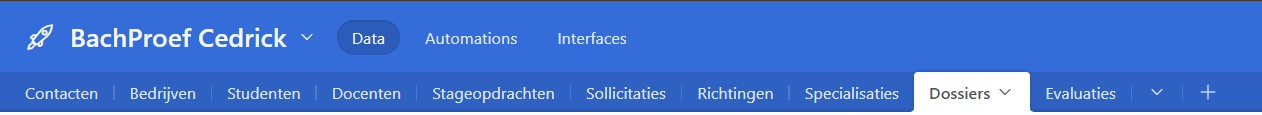
\includegraphics[width=\linewidth]{methodologie/Airtable_tables.jpg}
    \caption{Tables in Airtable.}
    \label{fig:meth_airtable_tables}
\end{figure}

Eens de vorige stap voltooid is, kunnen de attributen per tabel worden ingesteld. In Airtable stelt elke kolom van een tabel een attribuut voor. Om die redenen zijn er dus ook verschillende soorten velden, zoals een `Email` veld om e-mail bij te houden of een 'Phone' veld om een telefoonnummer bij te houden. Een klein verschil met Podio is dat Airtable geen speciaal veld om een adres op te slaan voorziet. Dit is toch wel belangrijk en maakt het bijhouden van een adres minder eenvoudig, aangezien dit dus door een gewoon tekstveld moet gebeuren. \\

De twee belangrijkste types velden zijn het `Relationship` veld en het `Formula` veld. Zoals de naam impliceert, wordt het `Relationship` veld gebruikt om, net zoals in Podio, relaties te leggen tussen de verschillende tabellen. Relaties op zich zijn goed uitgewerkt in Airtable, in tegenstelling tot Podio worden ze direct aan beide kanten toegevoegd. Dit betekent dat als er bijvoorbeeld in de `Specialisaties` tabel een link gelegd wordt naar `Richtingen`, dan zal er ook automatisch een veld worden toegevoegd in de tabel van 'Richtingen'. Bovendien kan er net zoals in Podio gekozen worden of het veld één of meerdere referenties mag bevatten. Verder heeft Airtable ook nog het `Lookup` veld, waarmee een waarde uit een andere tabel kan worden weergegeven. Om dit in Podio te bereiken zou een calculatie veld gebruikt moeten worden. \\

Het 'Formula' veld is vergelijkbaar met een calculatieveld in Podio. Hiermee kunnen aangepaste formules gemaakt worden op basis van andere velden in dezelfde table. Bovendien ondersteunt het veld een groot aantal functies en operatoren, waaronder wiskundige, logische en tekstfuncties. Verder is ook conditionele logica zoals een 'if-else' structuur mogelijk binnen dit veld. Kortom is het dus een krachtig hulpmiddel voor gegevensverwerking binnen Airtable.  In de use case wordt dit type veld vooral gebruikt om de ID's van de verschillende tabellen te berekenen. \\
 
In figuur \ref{fig:meth_airtable_dossiersTable} is de uitgewerkte tabel voor de 'Dossiers' weergegeven, waarvan structuur van de opzet is nagenoeg dezelfde als die in Podio, op enkele verschillen na. Zo wordt voor de totaal score bijvoorbeeld gebruik gemaakt van een ander soort veld dan het `Formula` veld. In tegenstelling tot Podio ondersteunt het `Formula` veld geen loops, in plaats daarvan voorziet Airtable het `Roll-up` veld. Met dit veld kan een lijst met waarden, afkomstige uit een relatie, worden verwerkt. Zo wordt voor de totaalscore de som gemaakt van elke score bij de evaluaties en daarna gedeeld door 20. \\ 

\begin{figure}[ht]
    \centering
    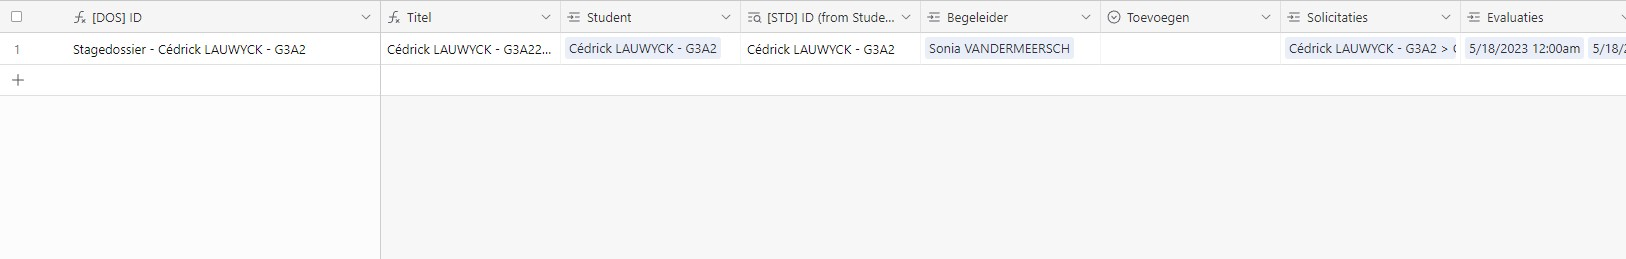
\includegraphics[width=\linewidth]{methodologie/Airtable_tableDossier.jpg}
    \caption{Uitgewerkte 'Dossiers' table in Airtable.}
    \label{fig:meth_airtable_dossiersTable}
\end{figure}


Na het instellen van de attributen, kan overgegaan worden tot de laatste stap in het bouw proces, namelijk automatisaties of workflows invoegen. In tegenstelling tot Podio, zitten deze wel ingebouwd in het platform en zijn ze gemakkelijk te bereiken via één simpele klik. In figuur \ref{fig:meth_airtable_automations} is te zien hoe ze zeer overzichtelijk worden weergegeven. Verder toont de figuur ook hoe een eenvoudige workflow is opgebouwd. In contrast met Podio is er geen apart gedeelte voor filters, maar zitten deze ingebouwd in de configuratie van de trigger,  daarna volgen direct de acties. Bovendien is er ook de optie om een workflow uit te testen, wat in Podio niet het geval is. \\

\begin{figure}[ht]
    \centering
    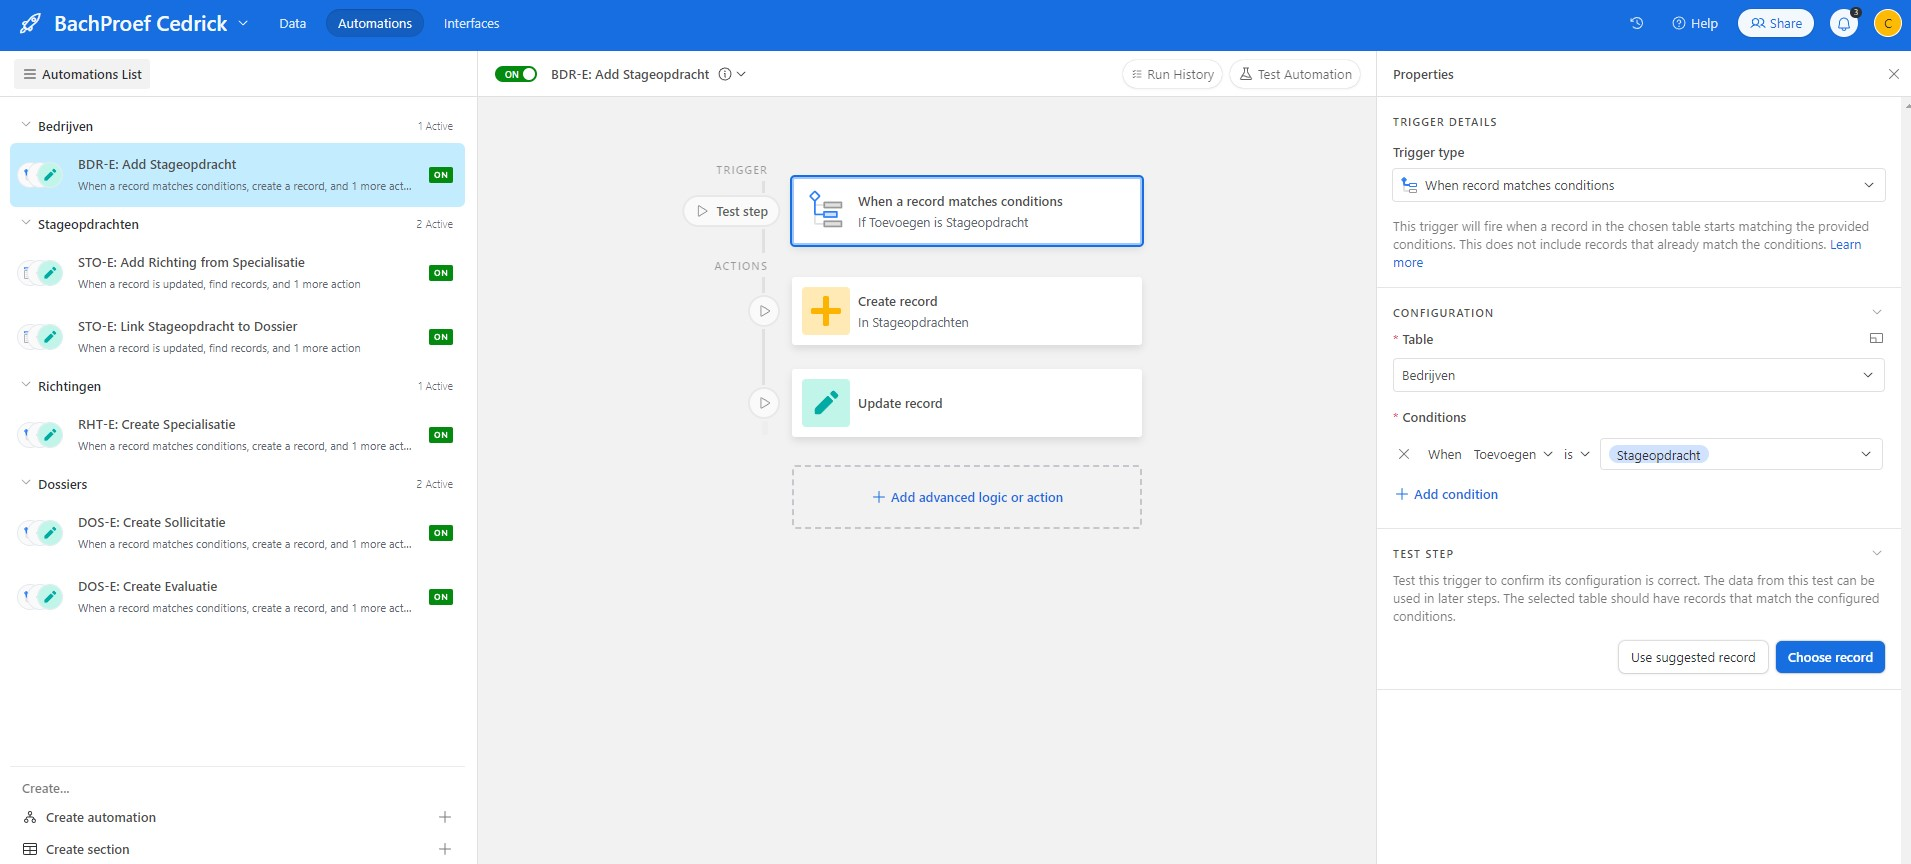
\includegraphics[width=\linewidth]{methodologie/Airtable_automations.jpg}
    \caption{Overzicht van automatisaties in Airtable.}
    \label{fig:meth_airtable_automations}
\end{figure}


Het omzetten tot pdf-bestand daarentegen is in Airtable niet zo eenvoudig dan als in Podio. Airtable voorziet in automatisaties namelijk geen optie om een pdf-bestand op te stellen, maar hier moet dit gebeuren via een extensie. Eerst en vooral is het belangrijk te vermelden dat de optie om extensies toe te voegen, ingebouwd zit in Airtable, wat in Podio niet het geval is. Er zijn verschillende extensies die het opmaken van een pdf-bestand verwezenlijken, zo heb je onder andere de `Page Designer` extensie, die ontwikkeld is door Airtable zelf. Hiermee kan je mooie templates opstellen en invullen met data uit de tabellen. Deze extensie beperkt zich wel tot een enkele pagina, wat dus niet altijd het geval is. Uiteindelijk werd voor deze use case gekozen om gebruik te maken van de `PDF Generator API` extensie. Ook hier wordt vooraf een simpele template opgesteld om vervolgens op te vullen met de gewilde velden uit de dossiers table. Ten slotte hoeven enkel nog de records die geconverteerd moeten worden, geselecteerd worden en kan een pdf-bestand gegenereerd worden. Dat pdf-bestand wordt dan toegevoegd in het `Attachments` veld van de records, zoals weergegeven in figuur \ref{fig:meth_airtable_dossiersAttachments}. Alhoewel hier dus geen automatisatie werd aangemaakt, is het wel degelijk mogelijk om een extensie uit te voeren via een automatisatie. Via de betaalde versie van Airtable kan men in automatisaties scripts toevoegen die het gebruik van extensies toelaat.  \\

\begin{figure}[ht]
    \centering
    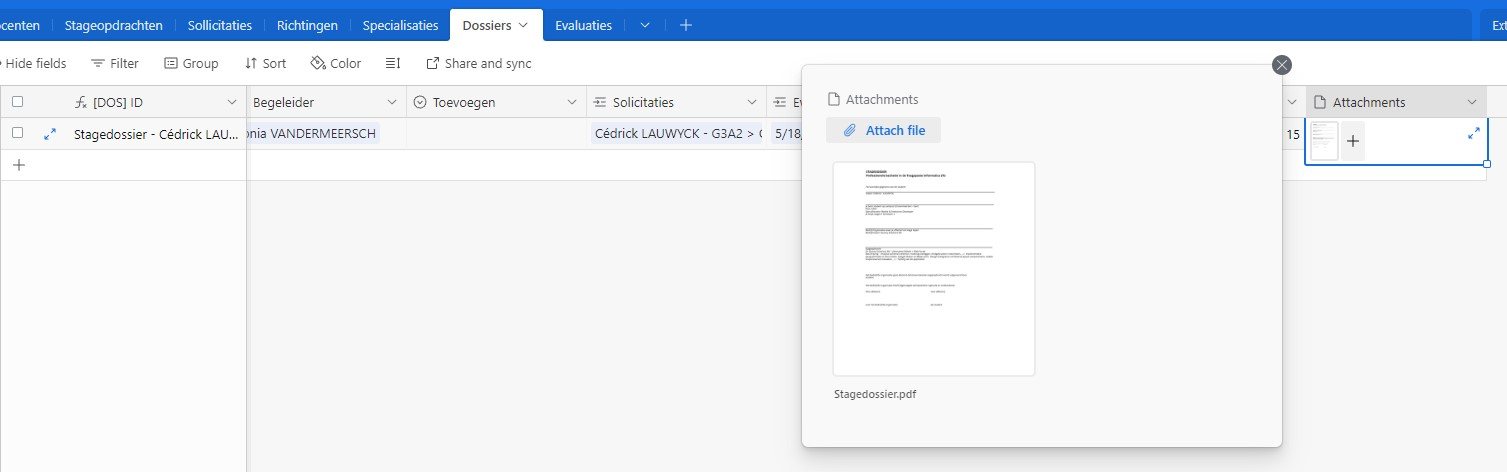
\includegraphics[width=\linewidth]{methodologie/Airtable_dossiersAttachments.jpg}
    \caption{pdf-bestand toegevoegd aan attachments veld in 'Dossiers' table na het uitvoeren van de workflow.}
    \label{fig:meth_airtable_dossiersAttachments}
\end{figure}

Ten slotte kan dus besloten worden dat het perfect mogelijk is om de use case uit te bouwen in Airtable. Ten eerste is het leggen van onderlinge relaties tussen verschillende tabellen zeer goed uitgewerkt, beter dan in Podio om dat er minder over nagedacht moet worden aan welke kant de relatie gelegd wordt. Op gebied van calculaties presteren Airtable en Podio even goed, toch is er voor Podio iets meer technische kennis over JavaScript nodig, terwijl dit in Airtable niet nodig is. Vervolgens is de gebruikerservaring in Airtable heel wat aangenamer dan die van Podio. Desondanks het feit dat in het algemeen een gelijkaardig aantal klikken nodig zijn om een bepaald doel te bereiken, wordt in Airtable nagenoeg geen tijd gebruikt voor het wisselen tussen tabellen, wat te danken is aan hun tabblad-structuur. Bovendien voorziet het platform ook een korte tutorial in het begin, waardoor een gebruiker gemakkelijk op weg geraakt. Verder is de gebruikersinterface of UI zeer mooi opgesteld. De belangrijkste functionaliteiten zijn eenvoudig te bereiken en de gebruiker wordt niet overrompeld door informatie. Een klein nadeel is wel dat er geen overzicht is voor de verschillende activiteiten die gebeuren binnen een workspace. Ten slotte werden tijdens het uitbouwen van de use case geen problemen tegengekomen, alle verliep vlot en de functionaliteiten werkten zoals behoort. \\

\newpage



% APPSHEET __________________________________________________________________________________________________________________________
\subsection{Google AppSheet} % TODO - AppSheet - OK

Nu ook Airtable onderzocht werd, kan overgegaan worden tot het tweede en laatste potentiële alternatief, namelijk Google AppSheet. Eerst en vooral is de structuur in Appsheet opmerkelijk anders dan in Podio of Airtable. Zoals weergegeven in figuur \ref{fig:meth_appsheet_structuur}, maakt het platform namelijk geen gebruik van workspaces en splitst het bovendien projecten op in databases en applicaties. Alhoewel dit iets mindere gebruikerservaring zorgt, omdat er vaak moet afgewisseld worden tussen de twee, heeft dit wel als voordeel dat een enkele database gebruikt kan worden door meerdere applicaties. Bij het aanmaken van een App is er net zoals bij Podio en Airtable de optie om data te importeren van een externe bron, namelijk de Google Drive van de gebruiker. Indien er voor gekozen wordt een blanco app aan te maken, zal Appsheet automatisch ook een achterliggende database creëren. \\

\begin{figure}[ht]
    \centering
    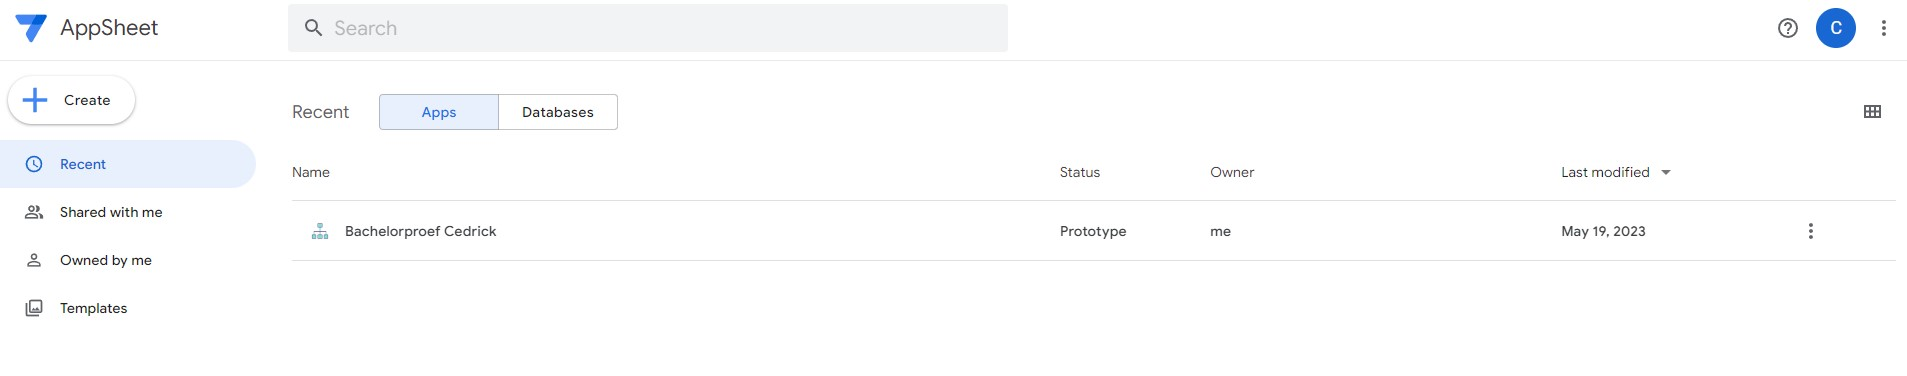
\includegraphics[width=\linewidth]{methodologie/Appsheet_structure.jpg}
    \caption{Structuur van AppSheet.}
    \label{fig:meth_appsheet_structuur}
\end{figure}

% uitleg structuur applicatie
Nadat de applicatie aangemaakt is, moet eerst de database correct geconfigureerd worden. In figuur \ref{fig:meth_appsheet_database} is te zien dat net zoals Airtable ook AppSheet met 'Tables' of tabellen werkt. Voor elk onderwerp uit de analyse wordt dus een tabel aangemaakt. Verder stellen ook de kolommen van de tabel terug de attributen voor, dus wordt voor elk attribuut een kolom aangemaakt. Net zoals bij Airtable en Podio zijn er een groot aantal verschillende velden waaruit gekozen kan worden om het type van een attribuut voor te stellen. In het algemeen bevat AppSheet zelfs meer types velden dan de vorige platformen. Toch ontbreekt er een zeer belangrijk veld, er is namelijk geen calculatie of 'Formula' veld. In Appsheet kunnen berekeningen of tekstverwerkingen niet ingesteld worden in de database zelf, maar gebeurt dit in het applicatie gedeelte, deze worden dus pas achteraf ingesteld. Daarnaast moeten de verschillende kolommen wel nog gelinkt worden met elkaar, dit gebeurt via het `Relationship` veld, dat zeer eenvoudig ingesteld kan worden. Verder heeft ook AppSheet een 'Look-up' veld dat toelaat om data uit een andere tabel weer te geven.

\begin{figure}[ht]
    \centering
    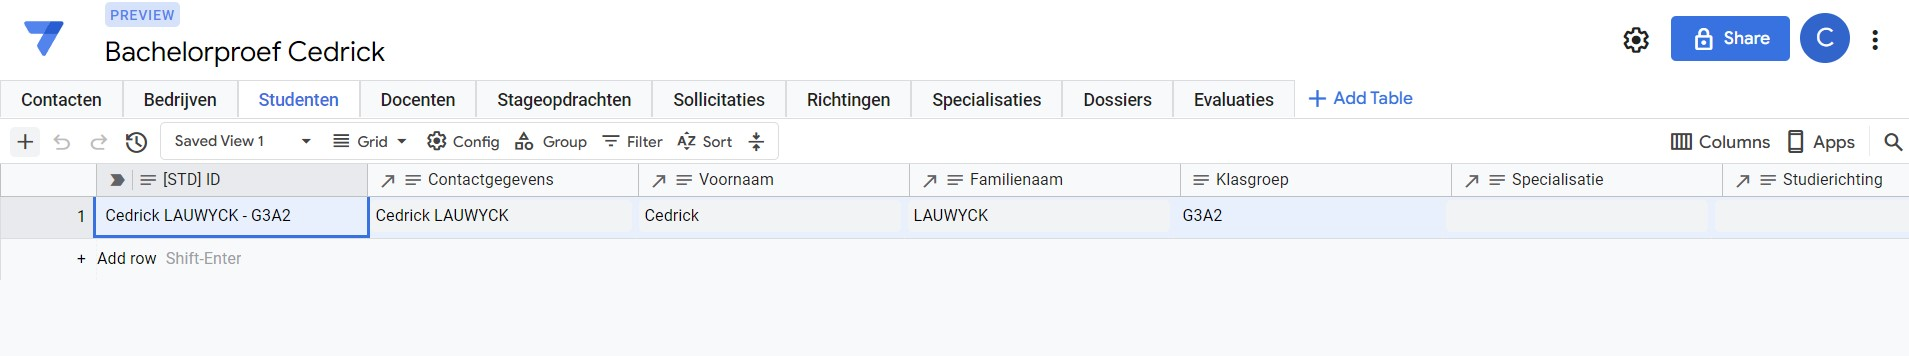
\includegraphics[width=\linewidth]{methodologie/Appsheet_database.jpg}
    \caption{Database in AppSheet.}
    \label{fig:meth_appsheet_database}
\end{figure}

Vervolgens kan overgegaan worden naar het applicatie gedeelte van het bouwproces, waar de formules worden toegevoegd. De structuur van dit deel wordt weergegeven in figuur \ref{fig:meth_appsheet_views} en gaat als volgt. Aan de rechterkant van het scherm wordt altijd een preview van de gebouwde applicatie getoond, de resterende ruimte wordt dan ingevuld met de verschillende configuratie opties. Om data weer te geven in de app, moet eerst een view aangemaakt en toegevoegd worden aan het menu. Een view omvat één tabel uit de database en geeft zijn data weer. Dit kan als verschillende vormen gebeuren, zoals als een gewone lijst of als een dashboard. Bovendien kan data die een 'Address' veld bevat ook weergegeven worden op een map door de ingebouwde Google Maps integratie die AppSheet voorziet. Uiteindelijk wordt dus voor elke tabel die werd aangemaakt in de vorige stappen een view gecreëerd. \\

\begin{figure}[ht]
    \centering
    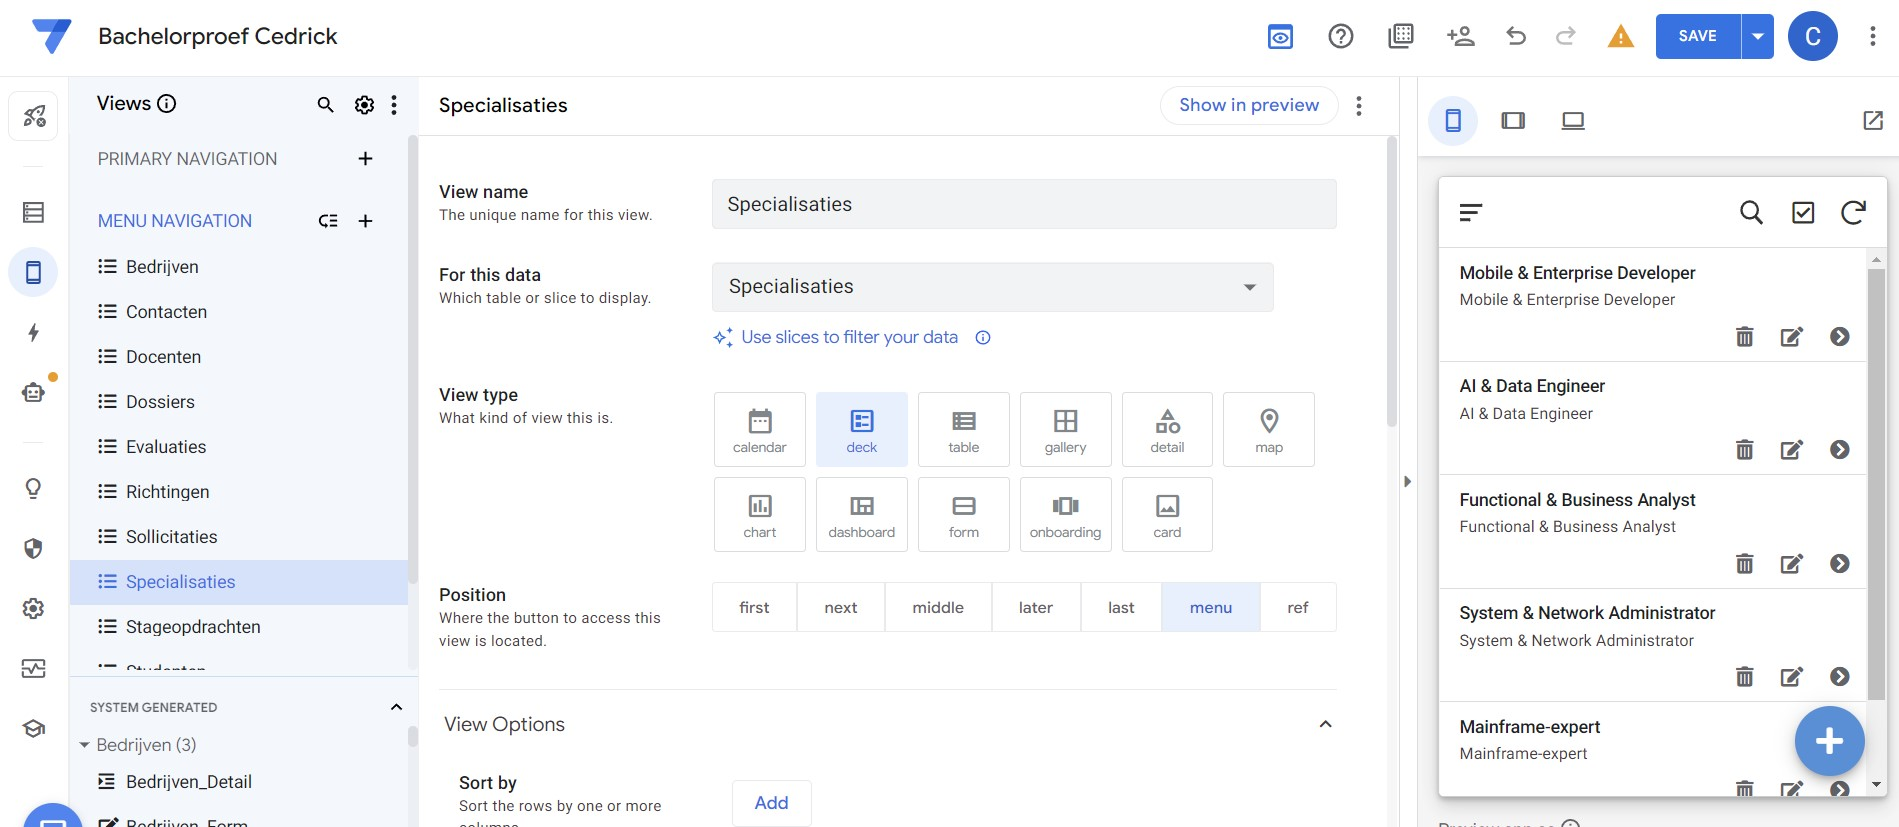
\includegraphics[width=\linewidth]{methodologie/Appsheet_views.jpg}
    \caption{Weergave van data in AppSheet.}
    \label{fig:meth_appsheet_views}
\end{figure}

Nu kunnen formules toegevoegd worden. De eerste stap hierbij is om bij elke tabel op de 'Regenerate schema' knop te klikken. Dit zorgt ervoor dat de verschillende database schema's in de applicatie up-to-date zijn met diegene in de database. Daarna kunnen de nodige formules ingevuld worden, deze zijn vergelijkbaar met formules in Microsoft Excel. In tegenstelling tot Podio kan in Appsheet elk veld als calculatieveld gebruikt worden. In figuur \ref{fig:meth_appsheet_formulas} is te zien hoe bij het invoeren van de calculaties er ook een `Expression Assistant` is die verschillende soorten voorbeeldformules weergeeft en ook de mogelijkheid bied om ze te testen. Daarnaast is er ook een 'Data Explorer' waarmee men gemakkelijk de nodige attributen kan invoeren. Uiteindelijk is het nog belangrijk om te vermelden dat berekeningen in AppSheet geen conditionele logica ondersteunen, wat toch wel een redelijk groot nadeel is. \\

\begin{figure}[ht]
    \centering
    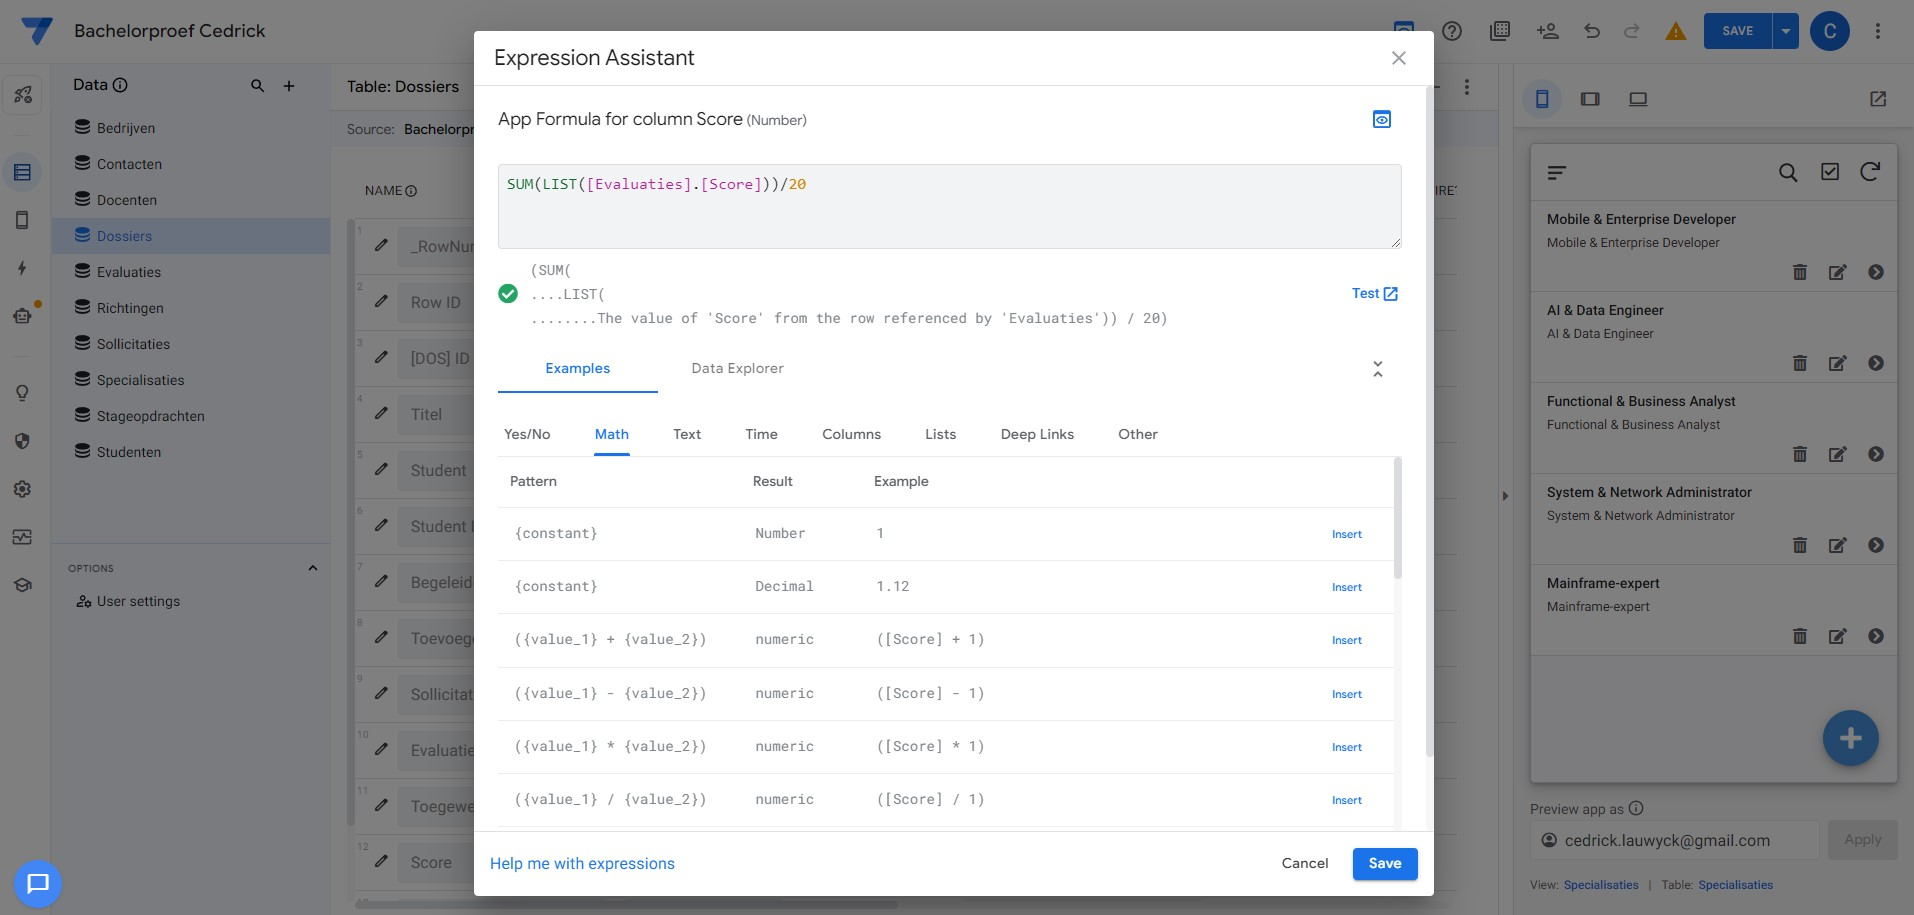
\includegraphics[width=\linewidth]{methodologie/Appsheet_formulaAssistant.jpg}
    \caption{Formules met `Expression Assistant` in Appsheet.}
    \label{fig:meth_appsheet_formulas}
\end{figure}

Een belangrijke opmerking bij Appsheet is dat het aanvullen van de database met gegevens in het applicatiegedeelte gebeurt. Hoewel de mogelijkheid bestaat om rijen toe te voegen in het database gedeelte, zullen op die manier de verschillende formules niet worden toegepast op de data. \\


% automatisaties
Nu kan terug overgegaan worden tot de laatste stap, automatisaties. In Appsheet hoeft enkel de automatisatie voor het omzetten naar pdf-bestand aangemaakt worden. De andere workflows zijn namelijk overbodig, omdat Appsheet al automatisch de mogelijke velden invult indien we op de 'Add'-knop klikken in de applicatie. Automatisaties zijn gemakkelijk te bereiken via een enkele klik op het `robot`-icoontje. Zoals te zien is in figuur \ref{fig:meth_appsheet_automations} wordt een automatisatie in AppSheet gedefinieerd door een zogenaamde `bot`, deze hebben hetzelfde concept als in Podio en Airtable, ze hebben namelijk een set van acties die worden uitgevoerd eens een bepaalde trigger geactiveerd wordt. Voor de use case wordt een bot gezet op de tabel dossiers, met als trigger een verandering in de kolom 'Toevoegen'.
Vervolgens wordt een actie toegevoegd om het dossier om te zetten naar een pdf-bestand. In tegenstelling tot Airtable zit deze functionaliteit net als Podio ingebouwd in AppSheet. Een nadeel is wel dat de gegenereerde pdf achteraf niet zomaar aan het dossier kan worden toegevoegd. Het wordt namelijk opgeslagen op een aparte plaats, zoals Google Drive of OneDrive. Om het bestand te linken aan het dossier, moet een formule worden toegepast op het 'Attachments' veld die verwijst naar de locatie of pad van het pdf-bestand. \\


\begin{figure}[ht]
    \centering
    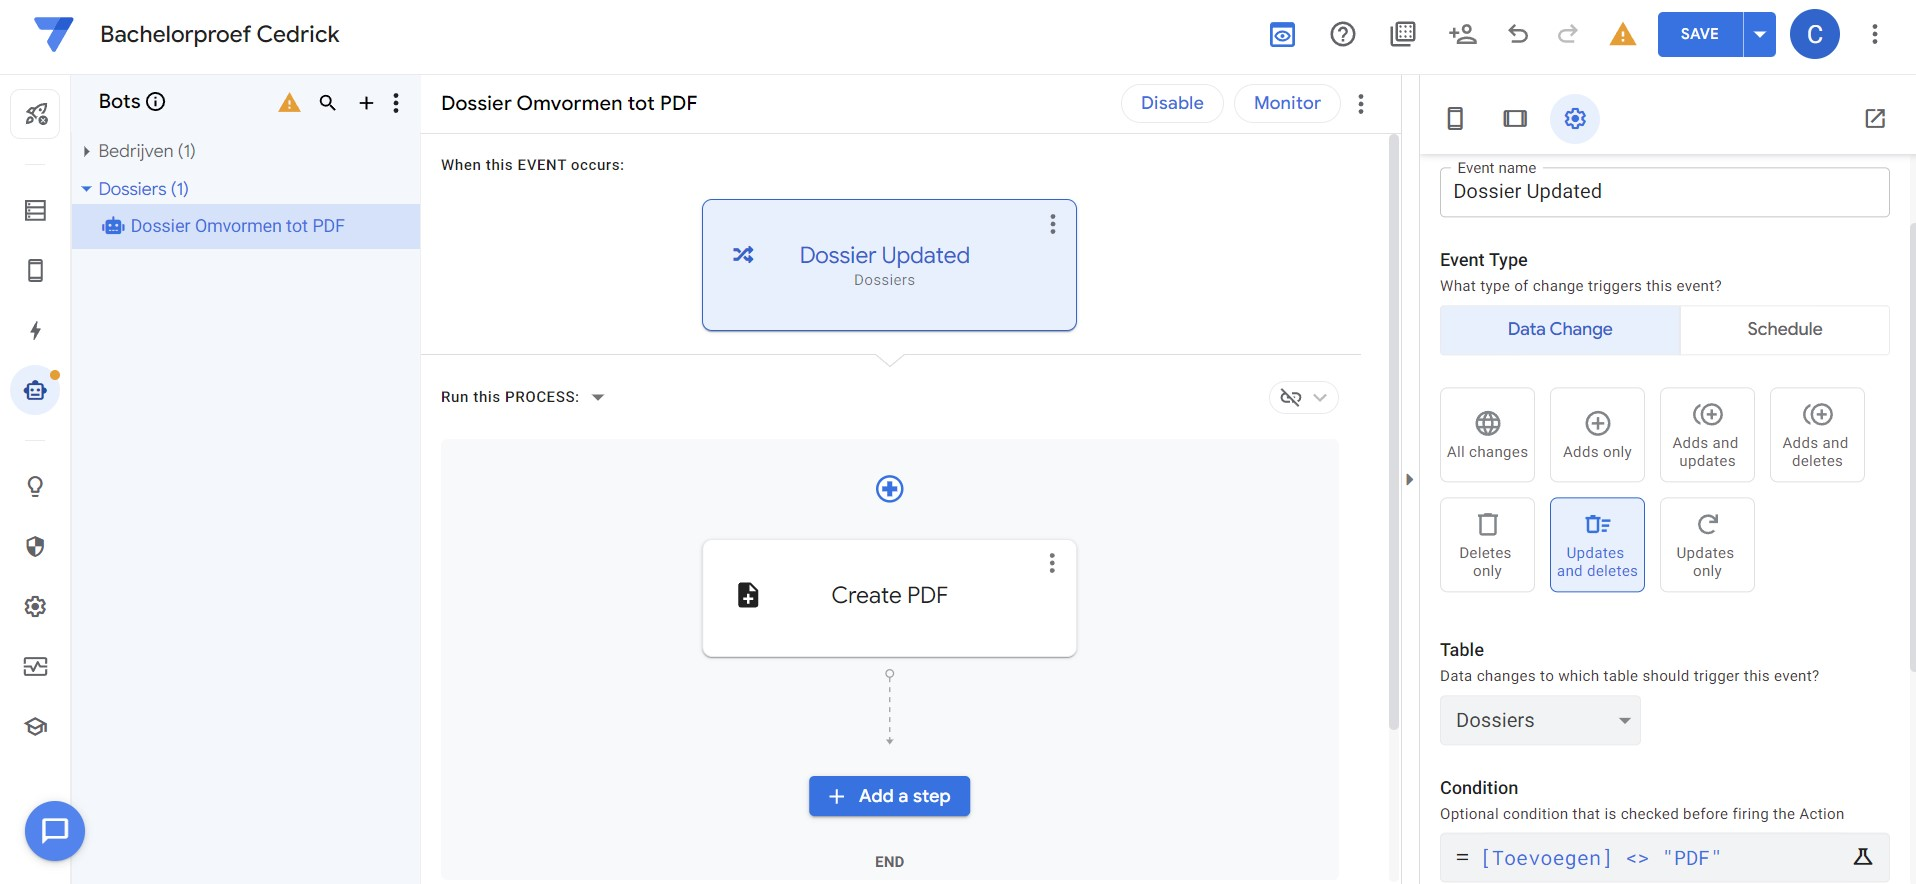
\includegraphics[width=\linewidth]{methodologie/Appsheet_automations.jpg}
    \caption{Automatisaties of 'bots' in Appsheet.}
    \label{fig:meth_appsheet_automations}
\end{figure}


Uiteindelijk is het dus ook perfect mogelijk om de use case uit te bouwen in Appsheet. Net zoals bij Airtable en Podio kunnen er relaties gelegd worden tussen de verschillende tabellen in de database. Verder is het feit dat calculaties op elk veld uitgevoerd kunnen worden een enorm pluspunt, toch is hun functionaliteit beperkter dan de calculatievelden in Podio. Op gebied van gebruikerservaring presteerde Appsheet het minst goed, er waren in het algemeen de meeste klikken\footnote{3 tot 5} en stappen nodig om een doel te bereiken. Daarnaast waren er ook nog extra klikken nodig, zoals het synchroniseren van de database schema's tussen de het applicatie- en databasegedeelte en het heen en weer gaan tussen de 2 delen. Desondanks het feit dat de UI van Appsheet duidelijk opgesteld is, kan ze als onoverzichtelijk overkomen op kleinere schermen, omdat alles dan meer op elkaar gezet wordt en er veel met scrollbars gewerkt moet worden. Ten slotte zijn er ook enkele problemen voorgekomen tijdens het uitwerken van de use case. Vaak waren dit synchronisatie problemen tussen de applicatie en de ingevulde formules. \\


